\documentclass[conference]{IEEEtran}
\IEEEoverridecommandlockouts
% The preceding line is only needed to identify funding in the first footnote. If that is unneeded, please comment it out.
% Template version as of 6/27/2024

\usepackage{cite}
\usepackage{amsmath,amssymb,amsfonts}
\usepackage{url} 
\usepackage{algorithmic}
\usepackage{graphicx}
\usepackage{textcomp}
\usepackage{xcolor}
\usepackage{float}
\def\BibTeX{{\rm B\kern-.05em{\sc i\kern-.025em b}\kern-.08em
    T\kern-.1667em\lower.7ex\hbox{E}\kern-.125emX}}

\begin{document}

\title{Inferno Tactics\\
% {\footnotesize \textsuperscript{*}Note: Sub-titles are not captured for https://ieeexplore.ieee.org and
% should not be used}
}

\author{\IEEEauthorblockN{1\textsuperscript{st} Shaurya Mathur}
\IEEEauthorblockA{\textit{Dept. of Computer Science \& Engineering} \\
\textit{University at Buffalo}\\
Buffalo, USA \\
smathur4@buffalo.edu}
\and
\IEEEauthorblockN{2\textsuperscript{nd} Shreyas Bellary Manjunath}
\IEEEauthorblockA{\textit{Dept. of Computer Science \& Engineering} \\
\textit{University at Buffalo}\\
Buffalo, USA \\
sbellary@buffalo.edu}
}

\maketitle

\begin{abstract}
    In this project, Inferno Tactics, we explore the integration of Reinforcement Learning (RL) with Deep Learning (DL) to develop a proactive system for wildfire prediction and verification using satellite imagery and spatio-temporal data. The system is structured into two interconnected modules. The first module leverages a deep learning model trained on historical wildfire patterns and Earth Engine satellite data to forecast potential wildfire events — predicting both the likely date and geographic location of ignition. Building on this, the second module introduces a reinforcement learning agent that interacts with a dynamic environment of evolving satellite data. The agent’s objective is to validate the predicted wildfire events by actively selecting and analyzing recent image sequences, maximizing verification accuracy through feedback-driven exploration. This multi-stage architecture harnesses the predictive power of DL and the decision-making strengths of RL to create a more robust and intelligent wildfire monitoring pipeline. While still under active development, preliminary results suggest that the RL-enhanced validation significantly improves the system’s ability to filter out false positives and deliver timely alerts for disaster management.
\end{abstract}

\begin{IEEEkeywords}
wildfire, gym, deep learning, reinforcement learning
\end{IEEEkeywords}

\section{Introduction}

Wildfires are increasingly becoming a global threat, with rising temperatures and shifting climate patterns contributing to their frequency and intensity. These fires not only devastate ecosystems but also endanger human lives and infrastructure. Traditional methods of wildfire detection and response often rely on environmental monitoring and sensor-based data; however, these approaches are largely reactive and struggle to provide timely and strategic interventions over vast, unmonitored regions.

\noindent
\textit{Inferno Tactics} explores a novel approach that integrates Deep Learning (DL) with Reinforcement Learning (RL) to both predict and plan for wildfire events. The DL component analyzes satellite imagery and historical wildfire data to forecast the time and location of potential wildfire outbreaks. In parallel, the RL component simulates a dynamic environment where wildfires may occur, allowing an intelligent agent to learn optimal mitigation strategies through trial-and-error interactions. These strategies can involve decisions such as resource deployment, early evacuation planning, or the prioritization of firebreak construction.

\noindent
By modeling wildfire scenarios as a Markov Decision Process (MDP), the RL agent learns to make sequential decisions that aim to minimize long-term damage. This dual-system framework—combining predictive modeling with adaptive planning—seeks to enable a more proactive and automated wildfire management system.

\noindent
This report presents the current progress of the project, including the design and development of the initial models, challenges faced during implementation, and the roadmap for future enhancements. The objective is to demonstrate the feasibility of combining DL and RL for improving wildfire prediction, verification, and strategic response planning.

\section{Background and Motivation}

\subsection{Wildfires and the Need for Intelligent Response}
Wildfires are becoming increasingly destructive due to climate change, land-use patterns, and prolonged dry seasons. Traditional wildfire response mechanisms, while valuable, often rely on reactive strategies that lack foresight and scalability. In the face of rapidly spreading fires, there's a growing need for proactive and intelligent systems that not only predict the likelihood of wildfires but also simulate and learn effective mitigation responses in real-time.

\subsection{Simulating Wildfire Behavior with Real-World Data}
To study wildfire dynamics in a realistic setting, we have developed an interactive simulation environment using \texttt{React.js} and \texttt{three.js}. This simulation serves as a visual and behavioral model of wildfire propagation, incorporating real-world geographic data to enhance its accuracy.

\noindent
Specifically, we use Google Earth Engine APIs to fetch terrain elevation and land cover data, which are then integrated into the simulation. These attributes—along with wind speed and direction—play a crucial role in shaping how fire spreads. By grounding the simulation in actual Earth data, we aim to mimic plausible wildfire scenarios that are both visually intuitive and spatially accurate.

\subsection{Modeling Firefighting Agents via Reinforcement Learning}
At the core of our project is a Reinforcement Learning (RL) agent designed to develop and optimize wildfire mitigation strategies. We connect our React-based frontend to a custom Python-based \texttt{Gym} environment via WebSockets, enabling real-time interaction between the simulation and the RL backend.

\noindent
The initial agent we have developed simulates a \textit{helitack} unit—a helicopter-based firefighting strategy. Using the \texttt{Stable Baselines3} library, we train the agent to explore and learn optimal policies to suppress fires efficiently across different terrain and wind conditions. The agent's goal is to minimize the spread and damage caused by the fire over time, adapting its actions based on changing environmental dynamics.

\subsection{Motivation for Hierarchical Multi-Agent Planning}
While the helitack strategy is effective in certain scenarios, real-world wildfire mitigation often involves a combination of approaches, including fire trucks, aerial water drops, and firebreak construction. To simulate such complexity, we plan to extend our system using \textit{Hierarchical Reinforcement Learning (HRL)}.

\noindent
In this framework, high-level policies will determine which mitigation strategy (e.g., helitack, fire truck dispatch) to deploy, while lower-level agents execute specialized tasks based on the chosen strategy. This modular architecture enables coordinated planning, resource allocation, and scalable learning across different fire response techniques.

\noindent
Our motivation stems from building a generalized, adaptable simulation tool that can train agents capable of multi-modal disaster response. By modeling realistic wildfire environments and training agents through trial-and-error, we aim to develop an intelligent system that can assist human decision-makers in planning efficient, timely, and context-aware fire mitigation strategies.


% \begin{figure}[h!]
%     \centering
%     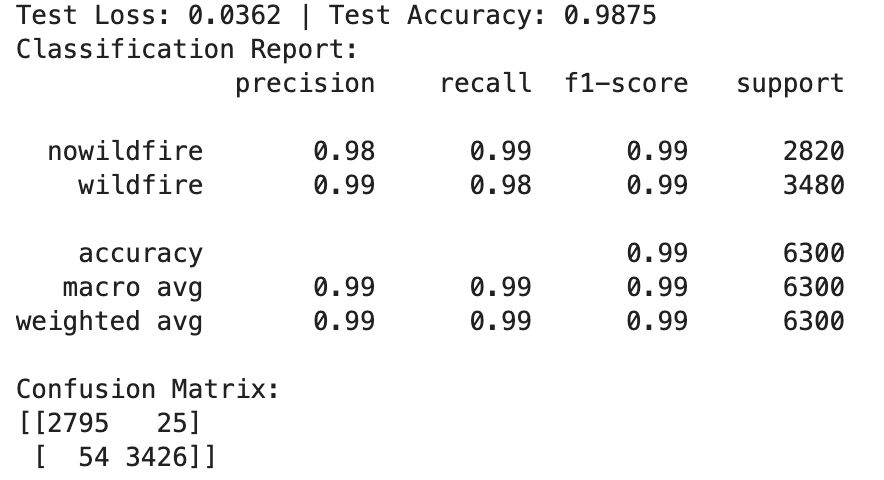
\includegraphics[width=0.5\textwidth]{result.jpeg}
%     \caption{Wildfire Classification Results.}
%     \label{fig:your_image_label}
% \end{figure}

% \begin{figure}[h!]
%     \centering
%     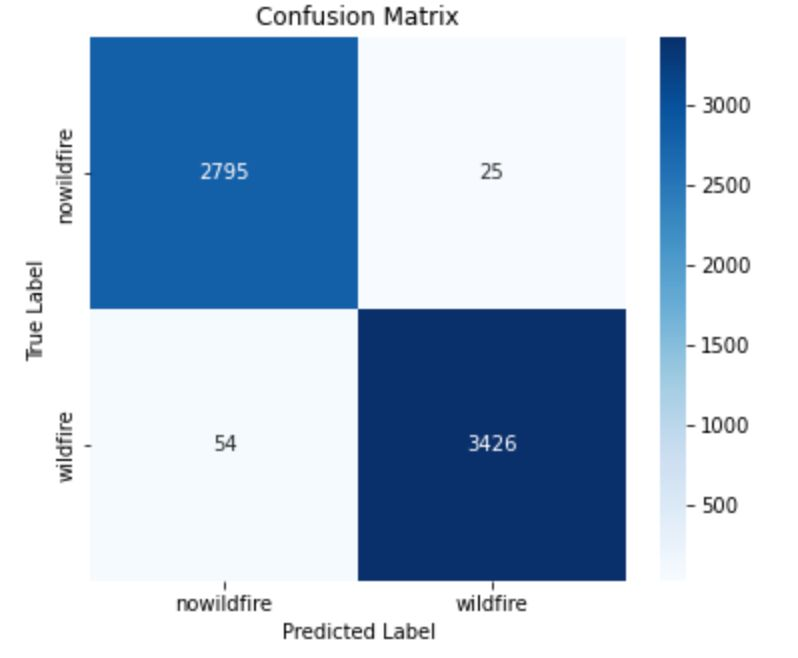
\includegraphics[width=0.5\textwidth]{cm.jpeg}
%     \caption{Confusion Matrix of Wildfire Classification Results.}
%     \label{fig:your_image_label}
% \end{figure}

\section{Preliminary Work}

Significant progress has been made in laying the foundation of the Inferno Tactics system. Our work spans the development of a 3D client simulation, the construction of a custom reinforcement learning (RL) backend, and the integration of real-world data sources to ensure a realistic training and evaluation environment. This section outlines the key components of our implementation so far.

\subsection{Client-Side Simulation Environment (React + Three.js)}
We developed an interactive simulation environment using \texttt{React.js} in combination with \texttt{Three.js} to visualize wildfire behavior in a 3D space. This browser-based frontend serves as a real-time visualization tool where:

\begin{itemize}
    \item Wildfires spread dynamically across a simulated terrain.
    \item Land cover types (e.g., forests, grasslands, barren regions) influence the spread rate and fire intensity.
    \item Environmental conditions such as elevation and wind direction are incorporated into the fire propagation logic.
\end{itemize}

\begin{figure}[h!]
    \centering
    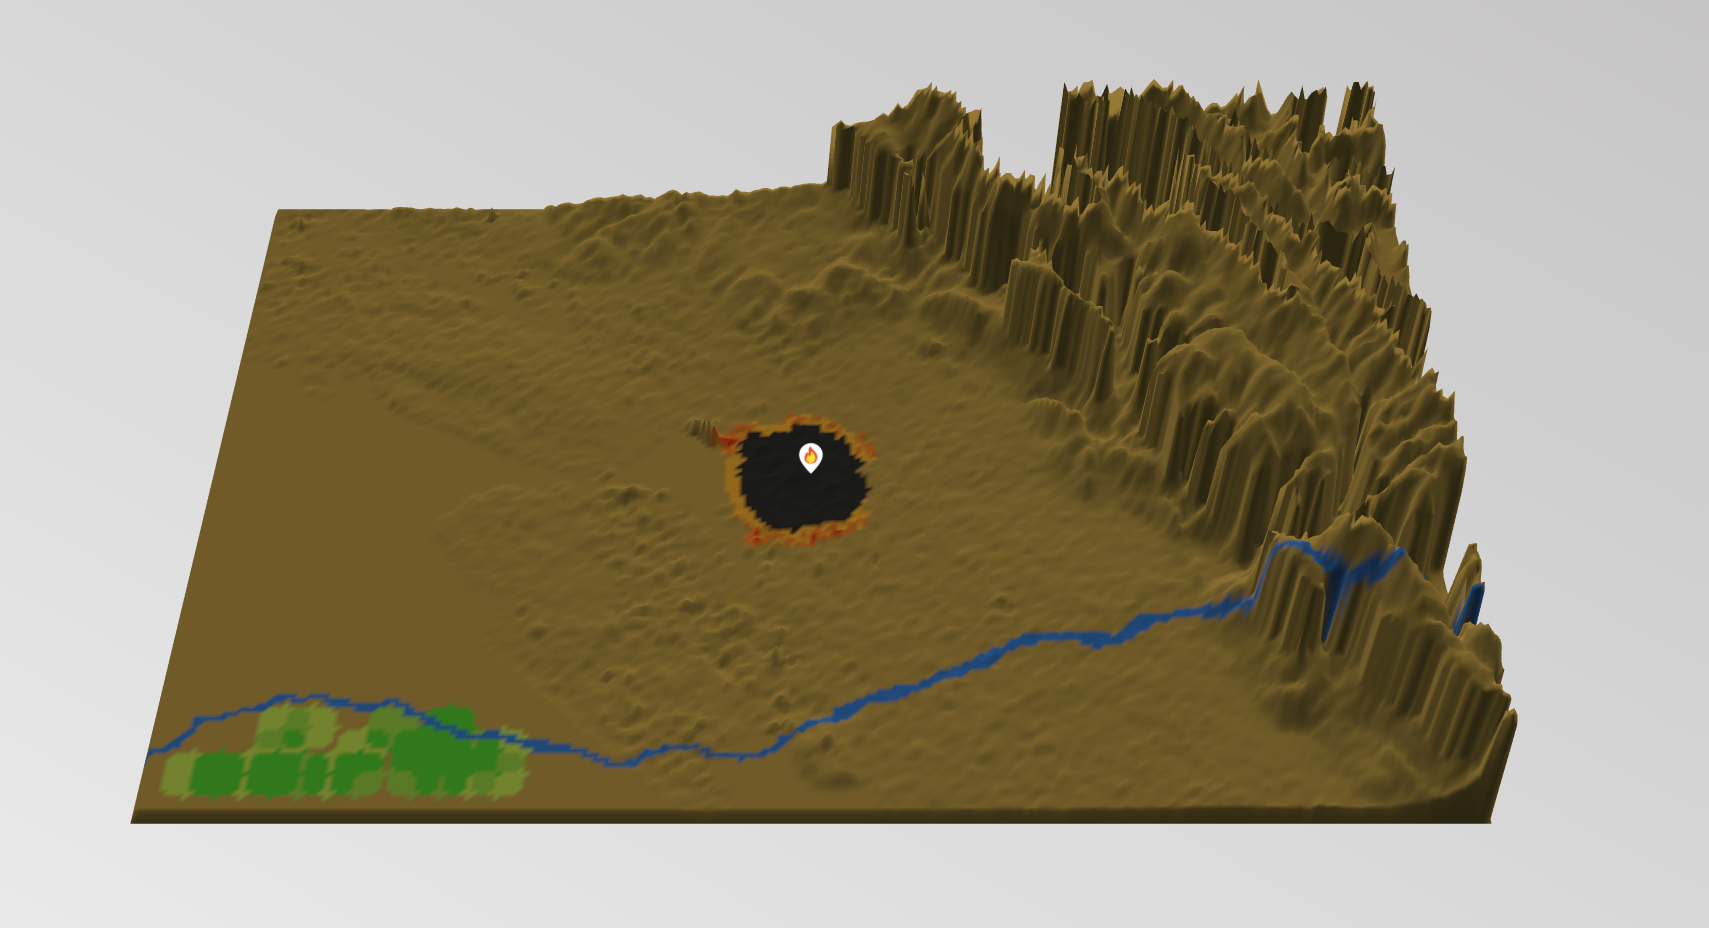
\includegraphics[width=0.5\textwidth]{sim.png}
    \caption{Wildfire Simulation Environment.}

\end{figure}

\noindent
The simulation is designed to support interaction with RL agents via live updates, reflecting both wildfire progression and agent interventions.

\subsection{Backend Architecture (Python, Gym, WebSockets)}
To interface with the simulation, we developed a custom \texttt{OpenAI Gym} environment in Python that models the wildfire spread logic and exposes a standardized RL interface.

\begin{itemize}
    \item The Gym environment is synchronized with the React frontend using \texttt{WebSockets}, allowing real-time bidirectional communication.
    \item Fire dynamics in the Gym environment replicate the frontend behavior to maintain consistency across training and visualization.
    \item The environment supports multi-step episodes where the agent can interact with the fire over a series of timesteps, receiving observations and rewards accordingly.
\end{itemize}

\subsection{RL Agent Development (Stable Baselines3)}
We have trained a baseline agent using the \texttt{Stable Baselines3} library. The agent simulates a \textit{helitack} (helicopter-based) firefighting strategy. Key aspects of this setup include:

\begin{itemize}
    \item The agent observes a spatial grid representing the fire map, land cover types, and wind patterns.
    \item Actions consist of moving to a particular coordinate and applying suppression in that region.
    \item Rewards are defined based on the amount of fire suppressed, area saved, and resource efficiency.
    \item The current policy is trained using \texttt{PPO} (Proximal Policy Optimization), with experiments underway to test other algorithms like \texttt{DQN} and \texttt{A2C}.
\end{itemize}

\subsection{Real-World Data Integration (Earth Engine SDK)}
To enhance realism and generalization, we integrated data from Google Earth Engine:

\begin{itemize}
    \item Elevation data is used to simulate terrain effects on fire spread.
    \item Land cover maps (e.g., MODIS, ESA WorldCover) help define fuel loads and flammability regions.
    \item This geospatial data is preprocessed and embedded into the simulation environment for both visual rendering and RL input representation.
\end{itemize}

\begin{figure}[h!]
    \centering
    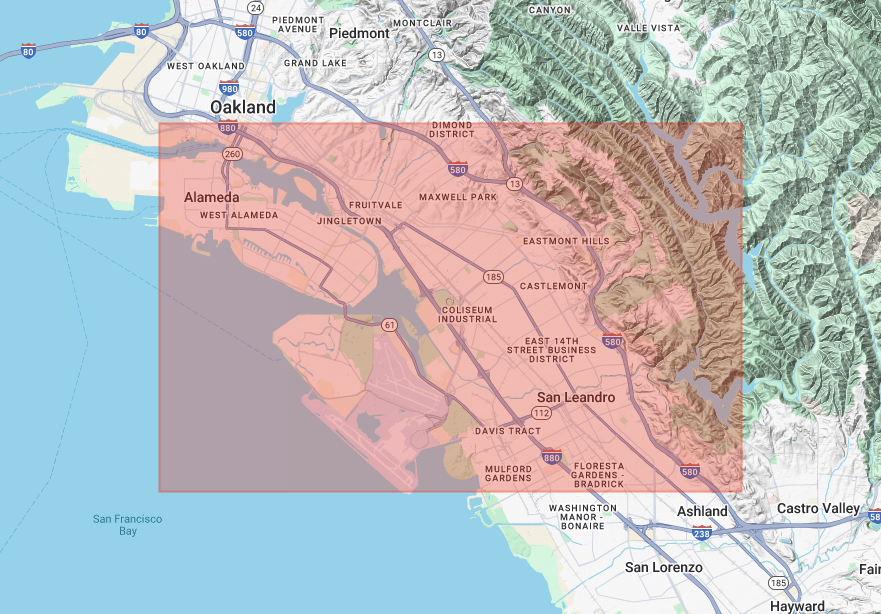
\includegraphics[width=0.5\textwidth]{terrain.png}
    \caption{Terrain View from EarthEngine.}
\end{figure}

\begin{figure}[h!]
    \centering
    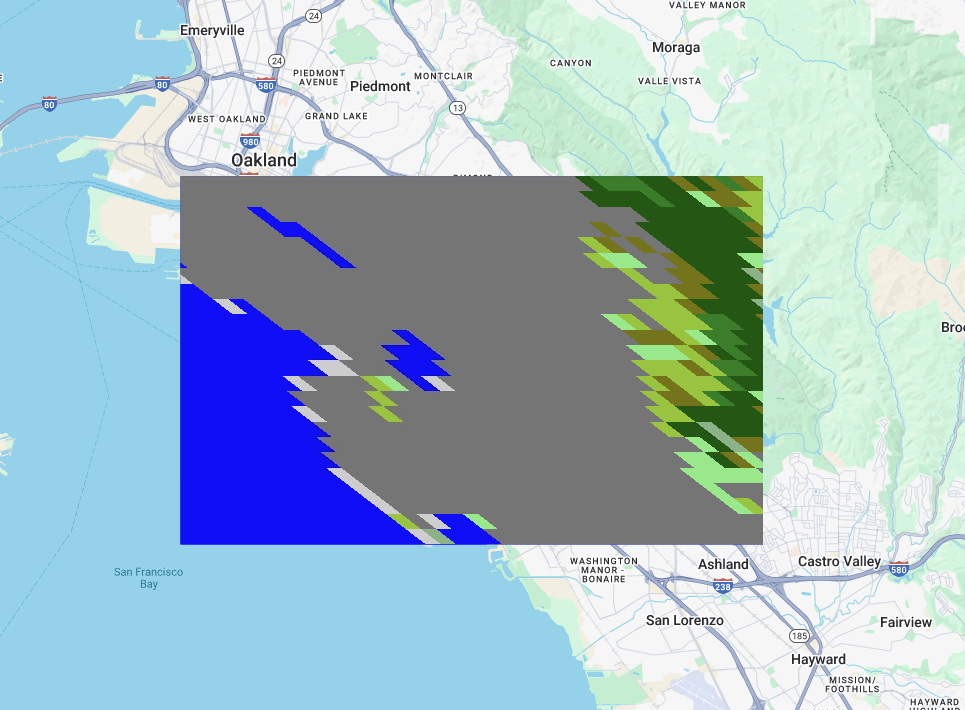
\includegraphics[width=0.5\textwidth]{landcover.png}
    \caption{Land Cover from EarthEngine.}
    
\end{figure}

\begin{figure}[h!]
    \centering
    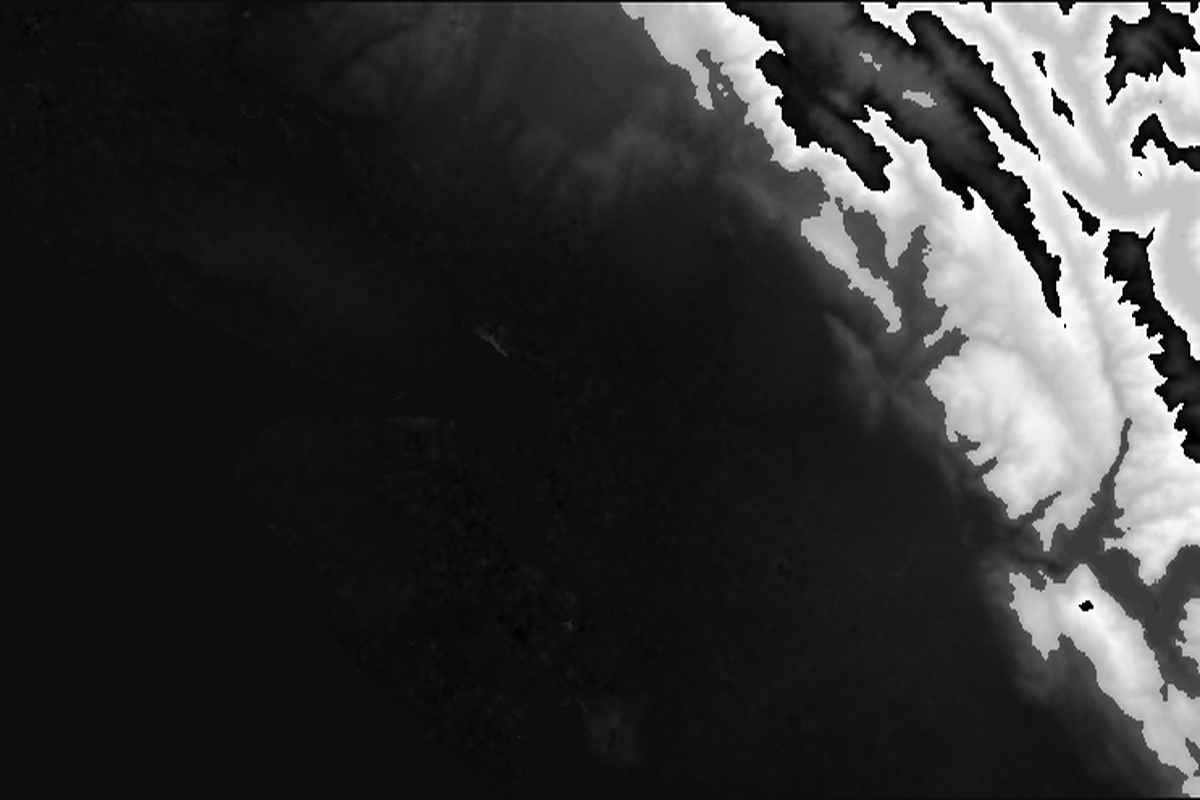
\includegraphics[width=0.5\textwidth]{heightmap.png}
    \caption{Heightmap of terrain depicting land elevations.}
\end{figure}

\noindent
This integration allows our simulation to reflect actual wildfire-prone locations, enabling future transfer learning from simulated to real-world geographies.

\subsection{Current Capabilities}
At this stage, our system is capable of:

\begin{itemize}
    \item Predicting and simulating the spread of wildfire on realistic terrain.
    \item Allowing a trained RL agent to interact with the fire and attempt suppression.
    \item Visualizing both fire progression and agent interventions in real time.
    \item Supporting expansion to additional agent types and hierarchical planning.
\end{itemize}

\noindent
Our preliminary work provides a strong technical foundation to explore advanced strategies such as hierarchical reinforcement learning and multi-agent coordination in future stages.

\section{Future Work}

While the current stage of the project has successfully established the foundational architecture and demonstrated promising initial results, several key enhancements are planned to extend the system’s capabilities, realism, and impact. These future steps are outlined below.

\subsection{Hierarchical Reinforcement Learning}
Our current system models a single firefighting strategy (helitack) through a single-agent RL approach. We aim to expand this to a multi-tiered control system using \textbf{Hierarchical Reinforcement Learning (HRL)}. In this framework:

\begin{itemize}
    \item A high-level policy will choose between multiple mitigation strategies, such as deploying fire trucks, helitacks, or constructing firebreaks.
    \item Low-level policies (sub-agents) will handle the specific execution of each strategy.
    \item This approach will allow the agent to operate at both strategic and tactical levels, improving overall adaptability and efficiency.
\end{itemize}

\subsection{Multi-Agent Coordination}
In real-world wildfire mitigation, coordination between multiple response units is essential. As a next step, we plan to implement a \textbf{multi-agent system} where:

\begin{itemize}
    \item Each agent represents a distinct firefighting unit (e.g., ground crew, aerial team).
    \item Agents may have overlapping but not identical observation spaces and action sets.
    \item Coordination and communication protocols will be explored using frameworks like MADDPG (Multi-Agent Deep Deterministic Policy Gradient).
\end{itemize}

\subsection{Policy Transfer to Real Geographies}
Currently, our training environments are based on simulated data generated from real-world maps. As the models mature, we intend to:

\begin{itemize}
    \item Fine-tune trained agents on historical wildfire case studies (e.g., California, Australia).
    \item Leverage transfer learning techniques to adapt policies across varying terrain and climate conditions.
    \item Validate agent performance using satellite data and fire event records.
\end{itemize}

\subsection{Real-Time Decision Support Tool}
A major goal of this project is to build a decision-support interface that can assist emergency response teams. Future development includes:

\begin{itemize}
    \item Deploying the simulation as a cloud-based tool with real-time updates.
    \item Allowing human operators to interact with the system and adjust RL agent recommendations.
    \item Incorporating user feedback to dynamically re-train or fine-tune models.
\end{itemize}

\subsection{Explainability and Trust in RL Decisions}
As we deploy RL in high-stakes decision-making scenarios, building trust in the agent’s choices is critical. Planned work includes:

\begin{itemize}
    \item Developing visualization techniques to explain agent decisions.
    \item Analyzing action trajectories and counterfactuals to understand failure cases.
    \item Using interpretable RL models or post-hoc explainability tools to aid human oversight.
\end{itemize}

\subsection{Integration with Government and NGO Systems}
Long-term, we envision this system being seamlessly integrated with wildfire management platforms used by:

\begin{itemize}
    \item Government agencies (e.g., CAL FIRE, NASA FIRMS) for real-time fire spread insights and mitigation planning.
    \item NGOs involved in environmental protection and disaster response for prioritizing interventions and resource deployment.
    \item Research organizations focused on climate-resilient infrastructure and AI-powered disaster forecasting.
\end{itemize}

\noindent
As a final output, the system generates a concise, human-readable one-page report using a fine-tuned large language model (LLM), summarizing the fire’s behavior, estimated spread, and recommended actions. This empowers field officers and policy makers to make fast, informed decisions without needing to interpret complex geospatial data.

\noindent
By continuing to refine and scale this pipeline, we aim to offer a robust, intelligent, and accessible decision-support framework to help tackle one of the world’s most urgent environmental threats.

\section{Bonus: Project Management Tool}
For this project, we utilized \textbf{Trello} as our project management tool to ensure structured progress tracking and clear communication. The project was divided into several milestones including data exploration, proposal drafting, basic and advanced model implementations, training, testing, and final presentation preparations.

Since our collaboration spanned both the reinforcement learning (RL) and deep learning (DL) parts of the project, both Trello boards were linked. Weekly tasks were clearly documented, enabling effective contribution tracking and synchronization between team members.

Key milestones included:

\begin{enumerate}
    \item[-] Project initialization
    \item[-] Data gathering and preprocessing
    \item[-] Initial model development
    \item[-] Advanced model enhancements
    \item[-] Training and validation of models
    \item[-] Evaluation and final adjustments
\end{enumerate}

\subsection{Project Management Screenshots}
Below are screenshots showcasing our Trello-based project management efforts:

\begin{figure}[H]
\centering
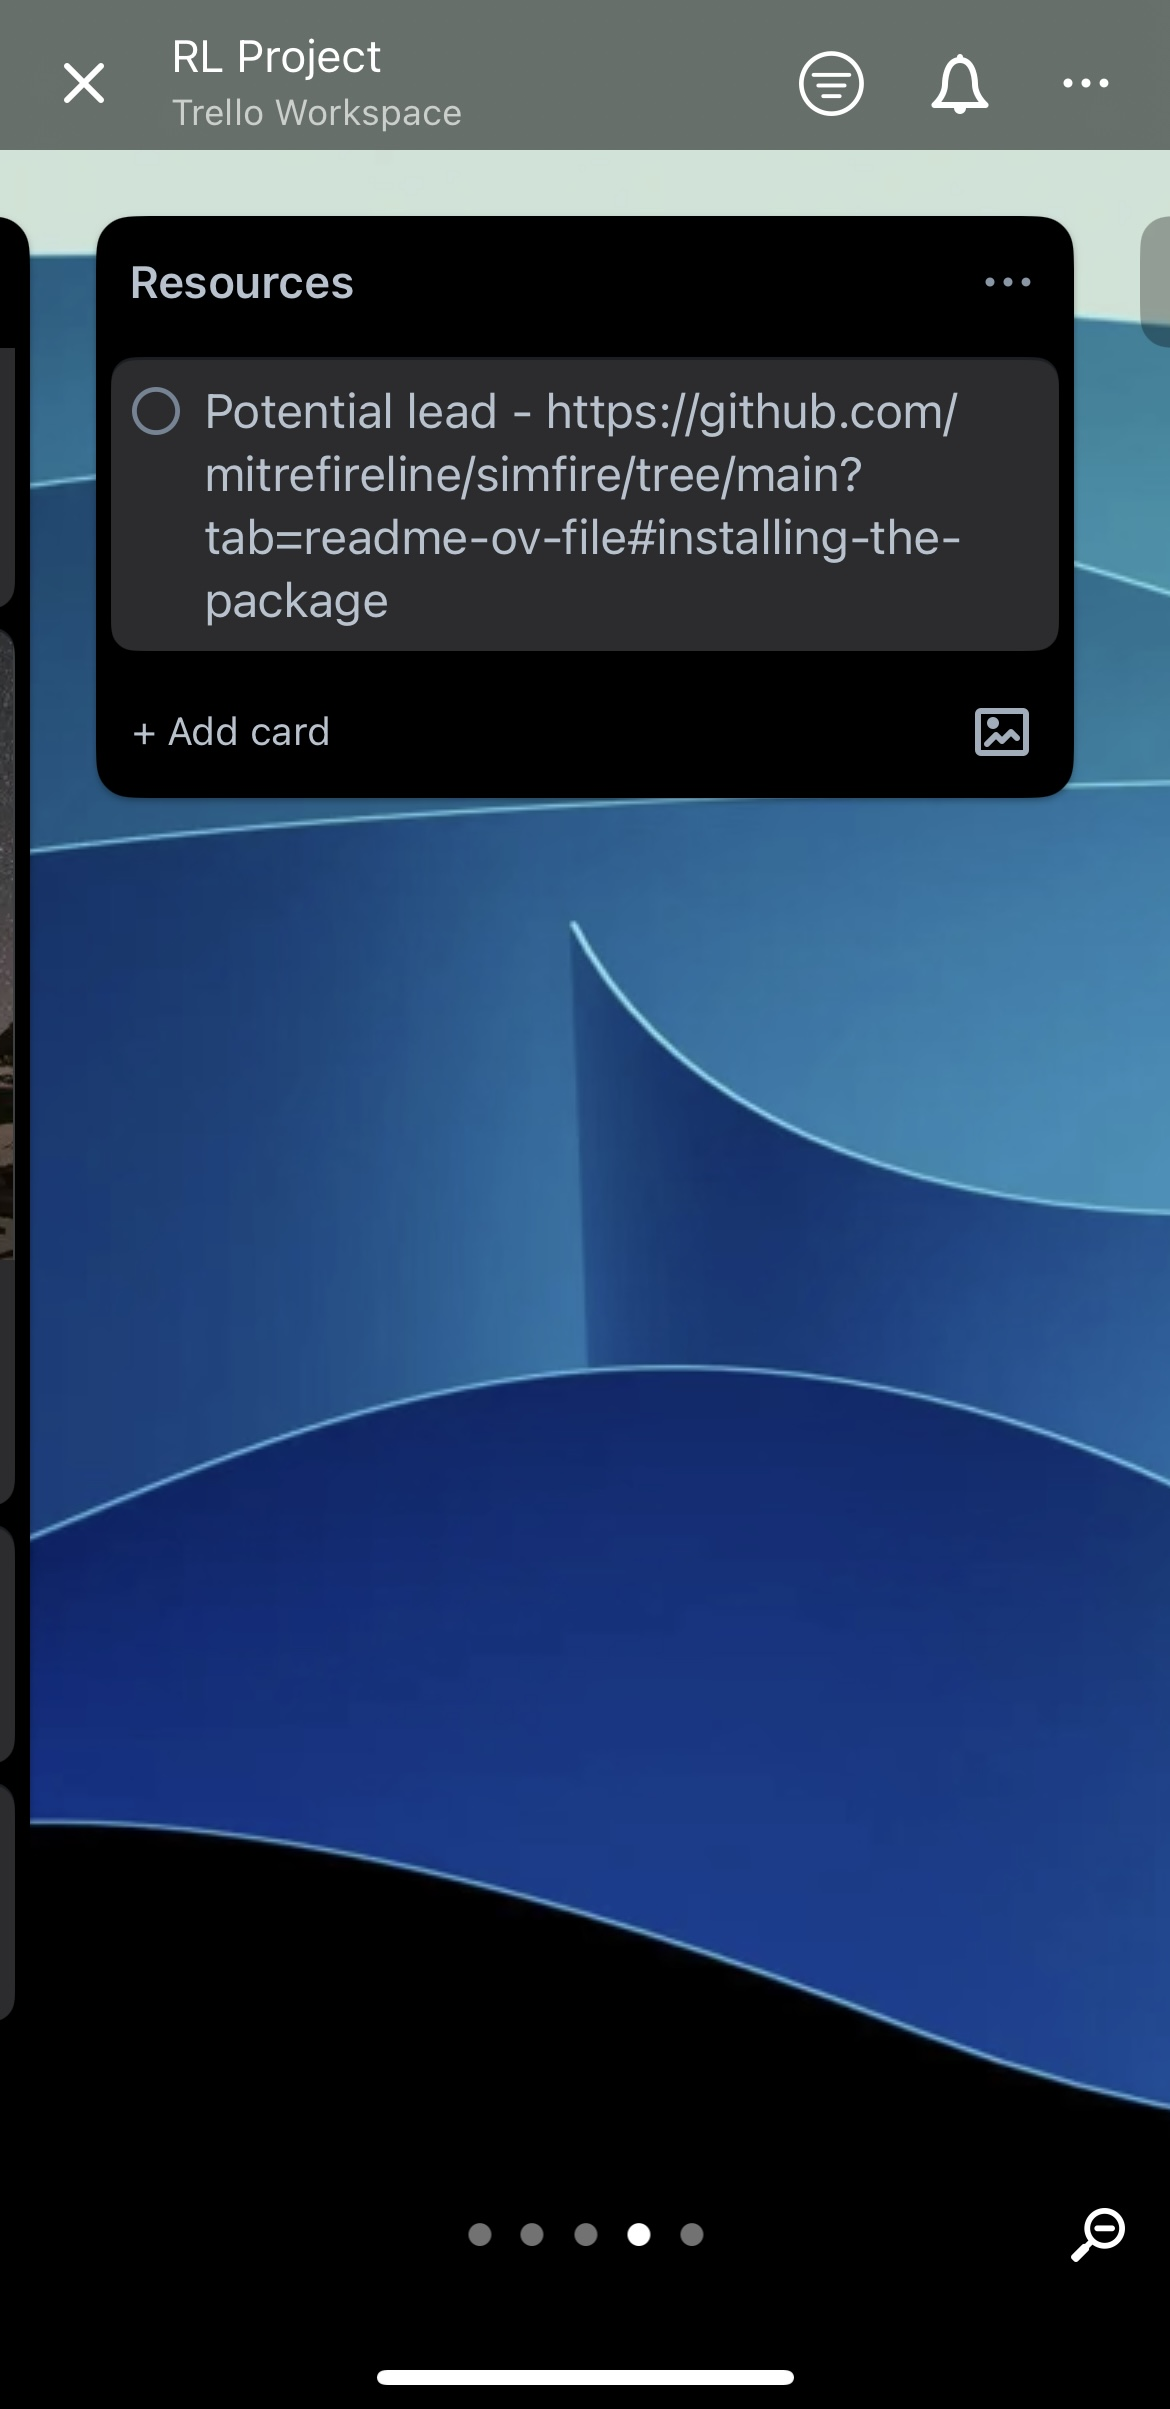
\includegraphics[width=0.2\textwidth]{1.jpg}
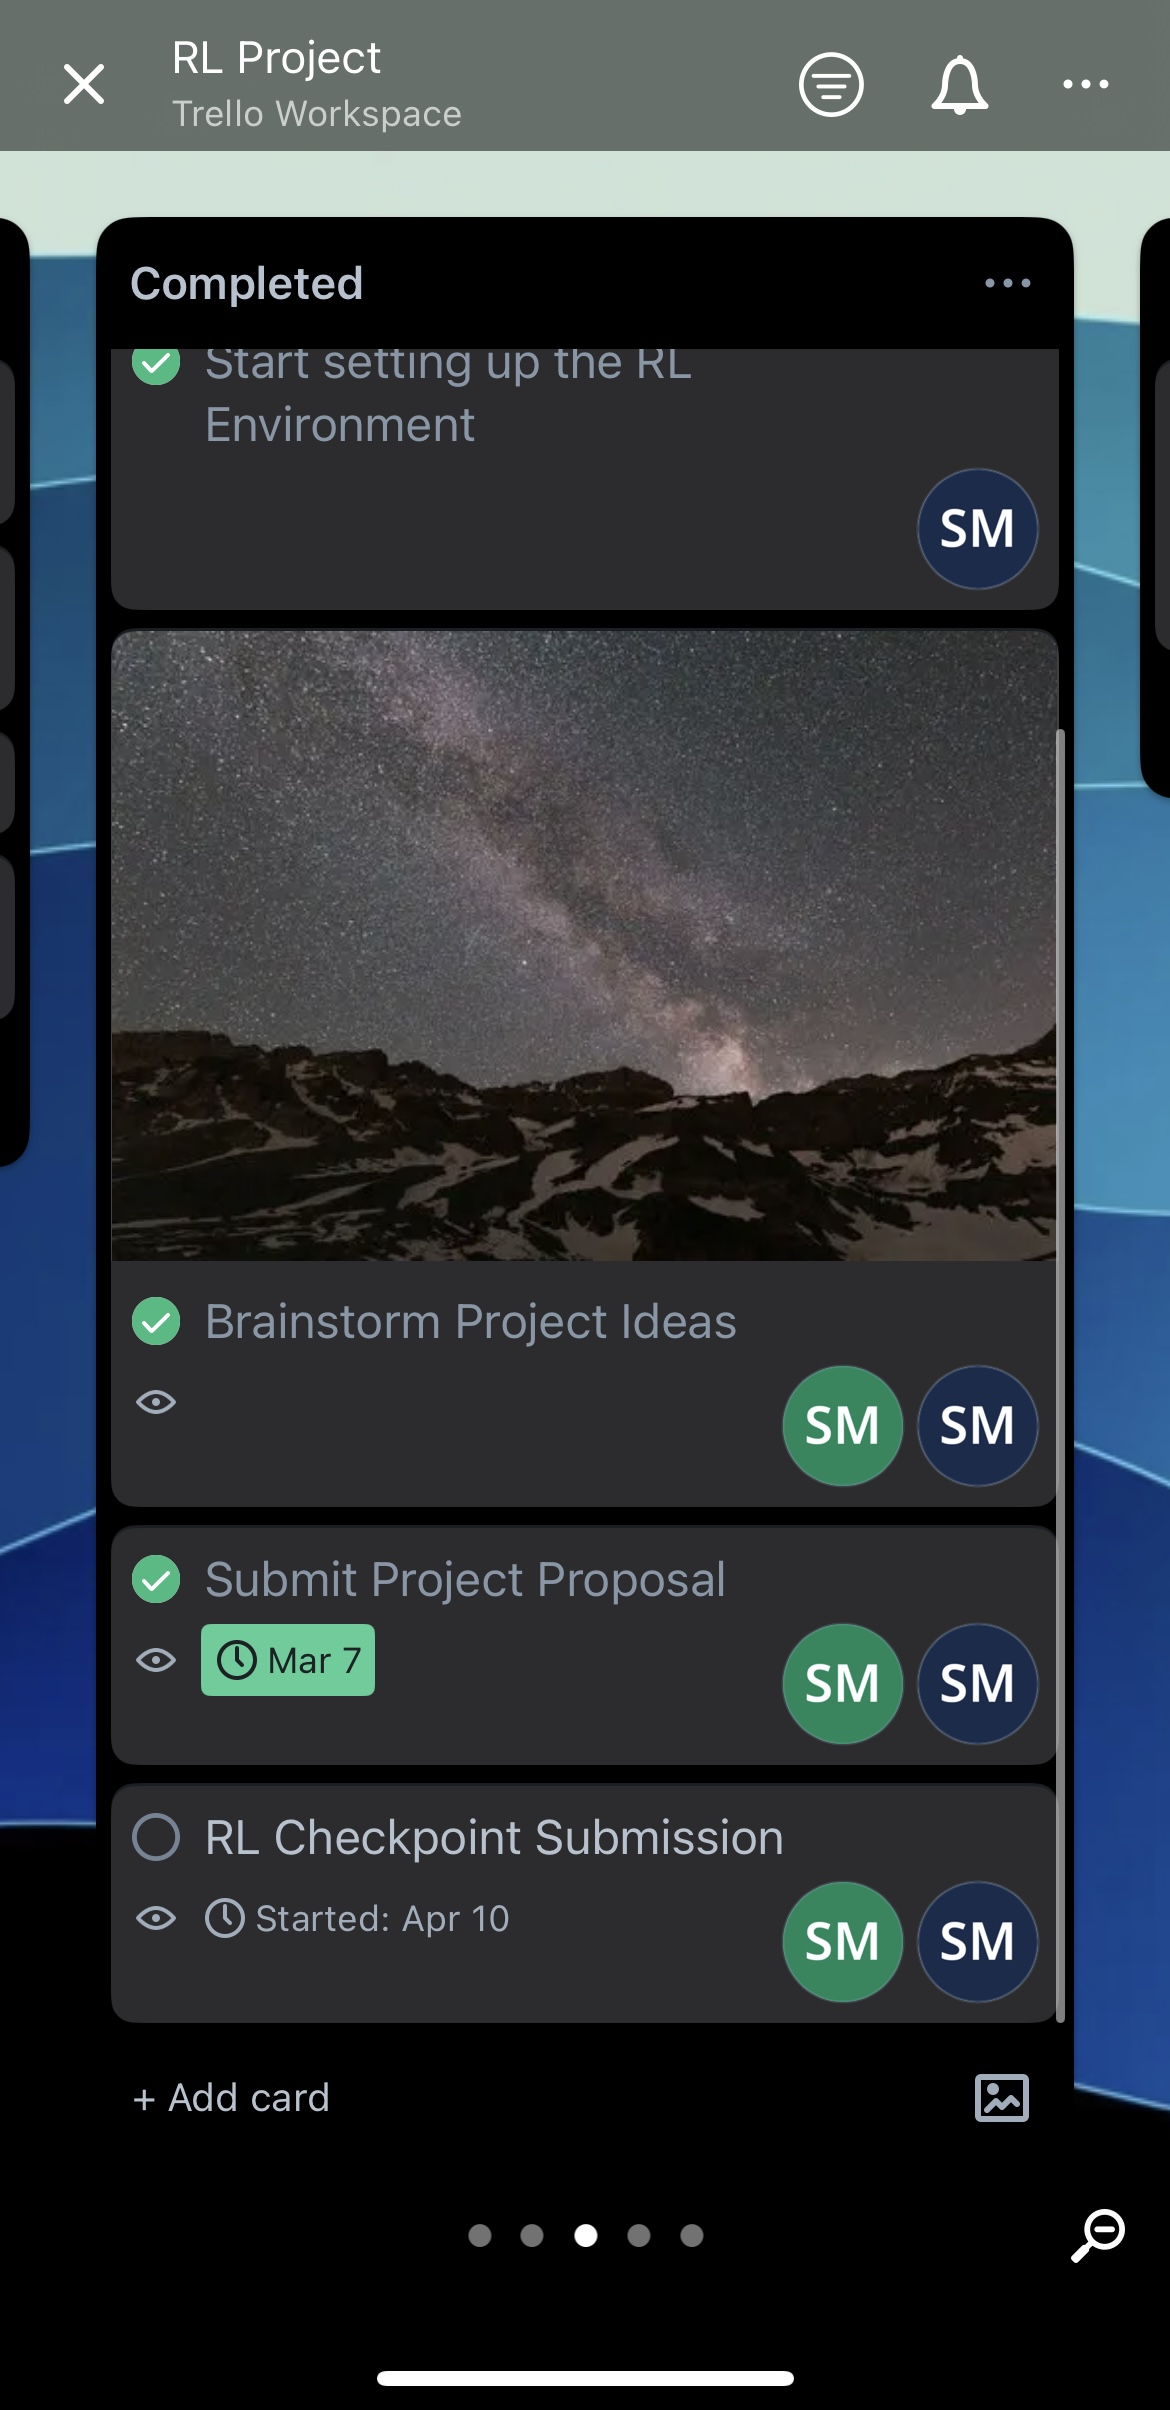
\includegraphics[width=0.2\textwidth]{2.jpg}
\end{figure}
\vspace{-0.7cm}
\begin{figure}[H]
\centering
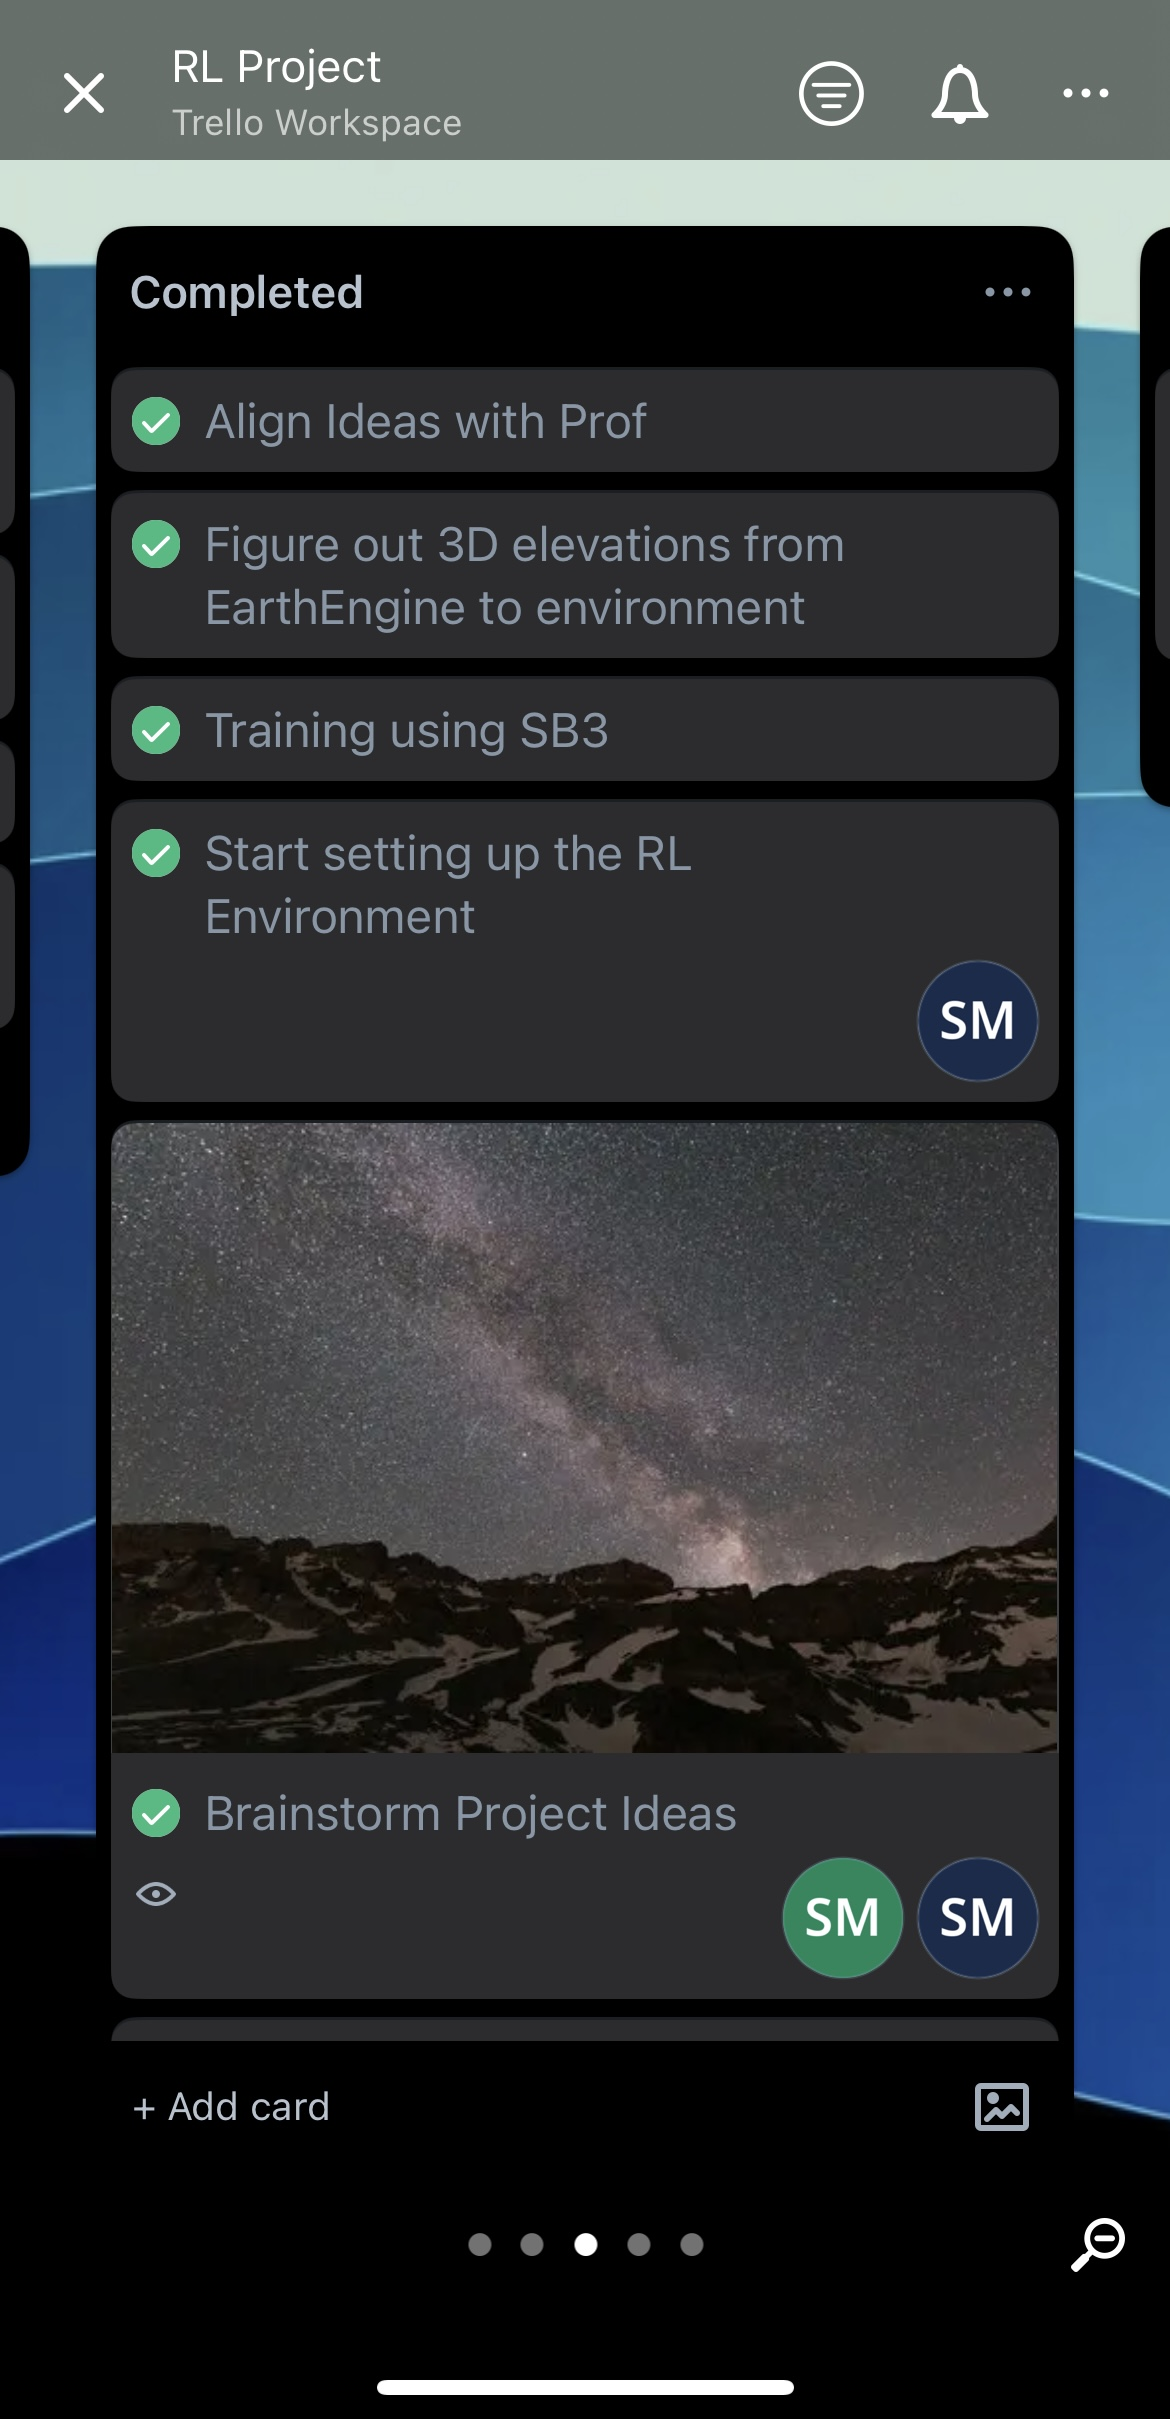
\includegraphics[width=0.2\textwidth]{3.jpg}
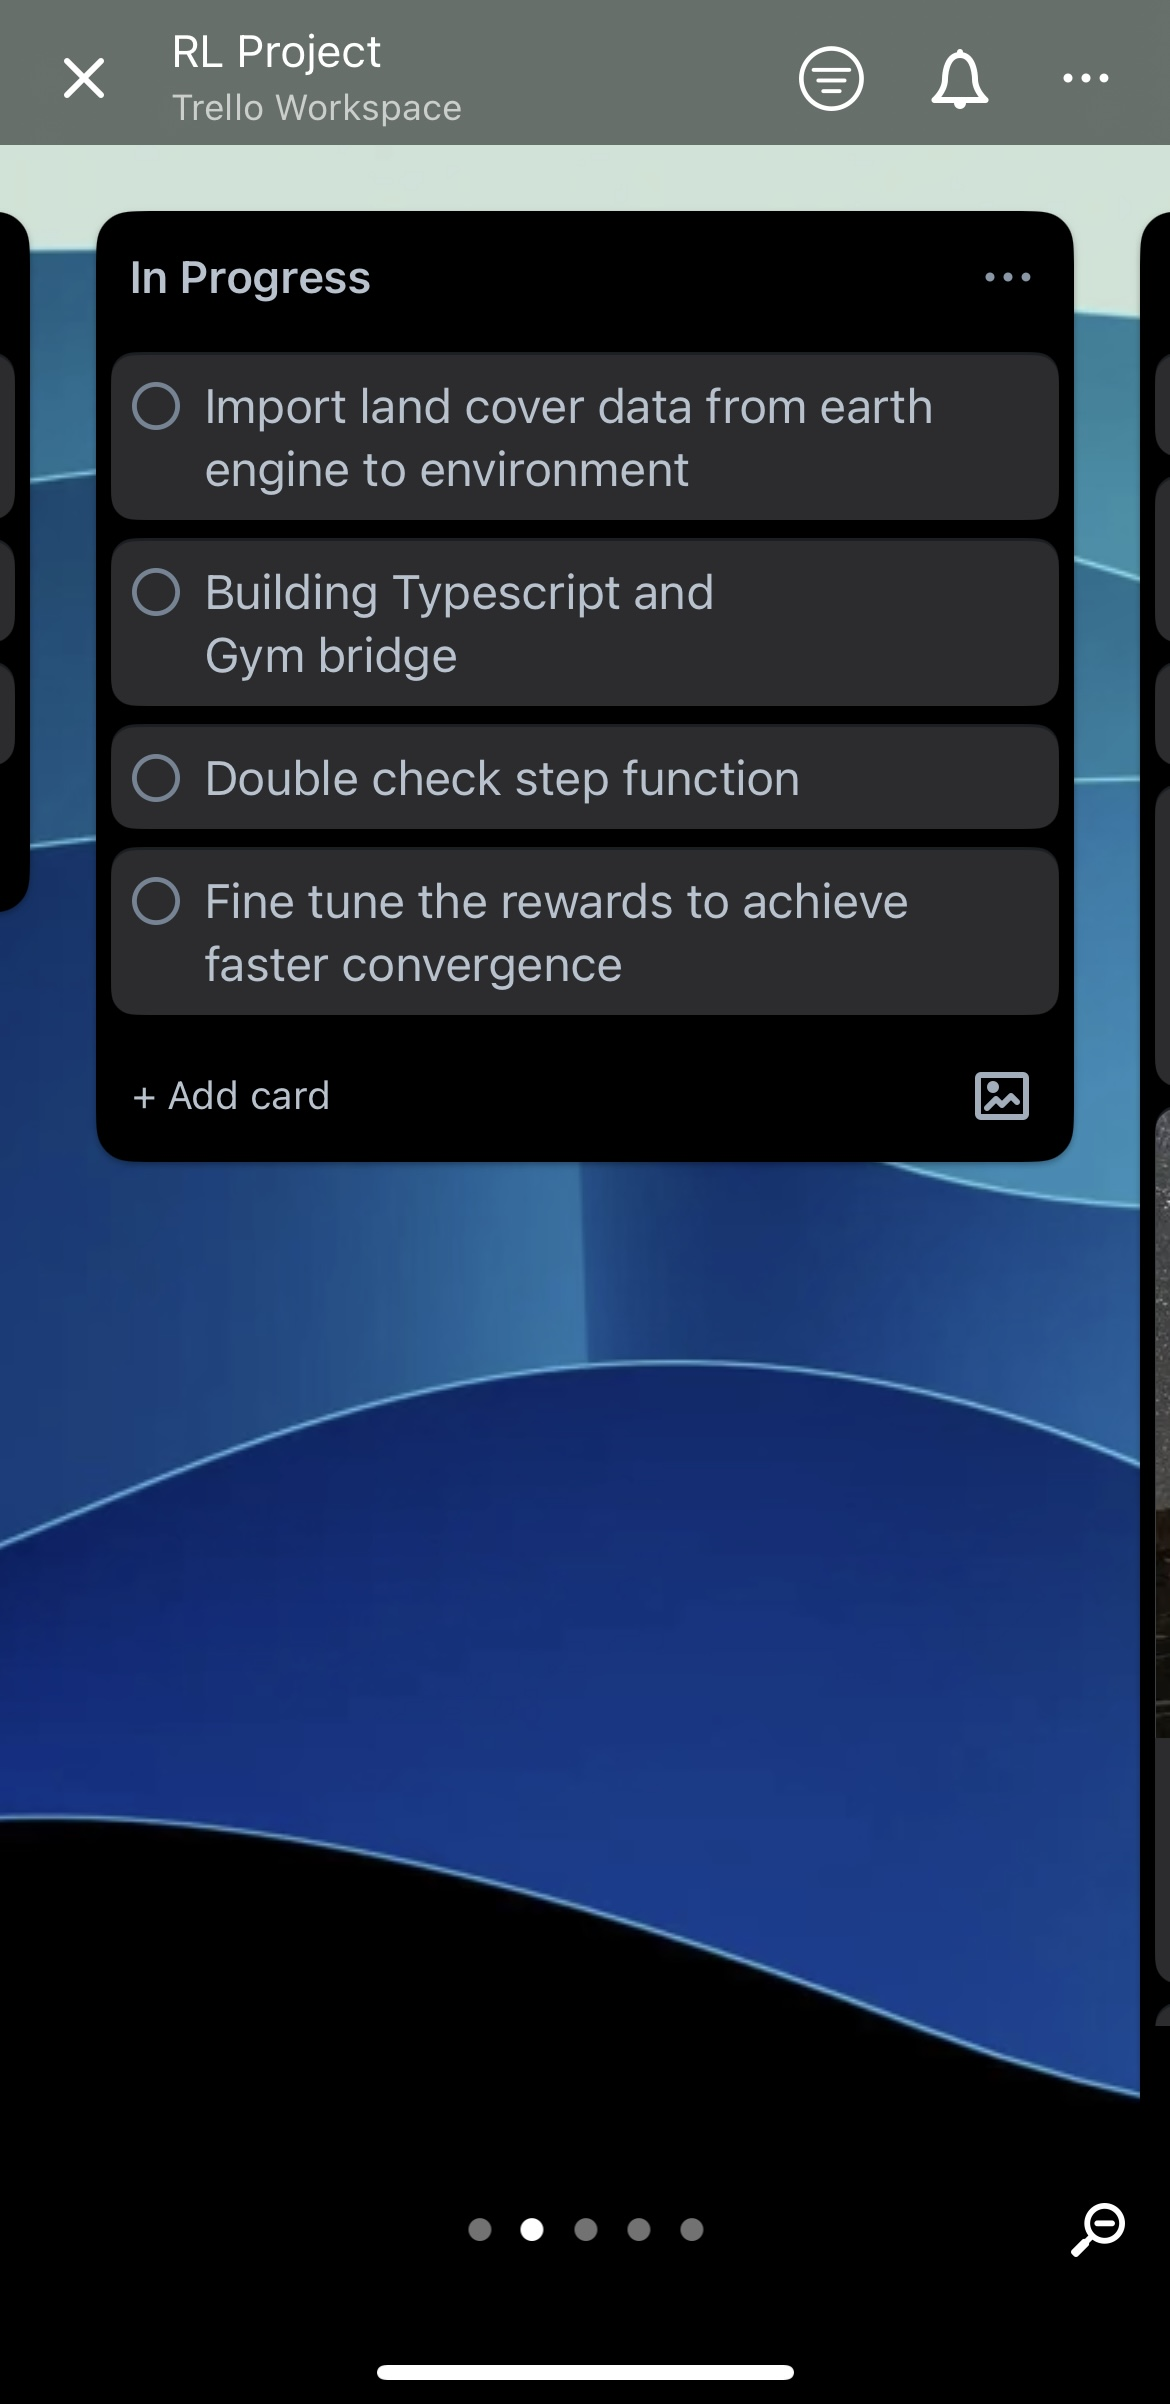
\includegraphics[width=0.2\textwidth]{4.jpg}
\end{figure}
\vspace{-0.7cm}
\begin{figure}[H]
\centering
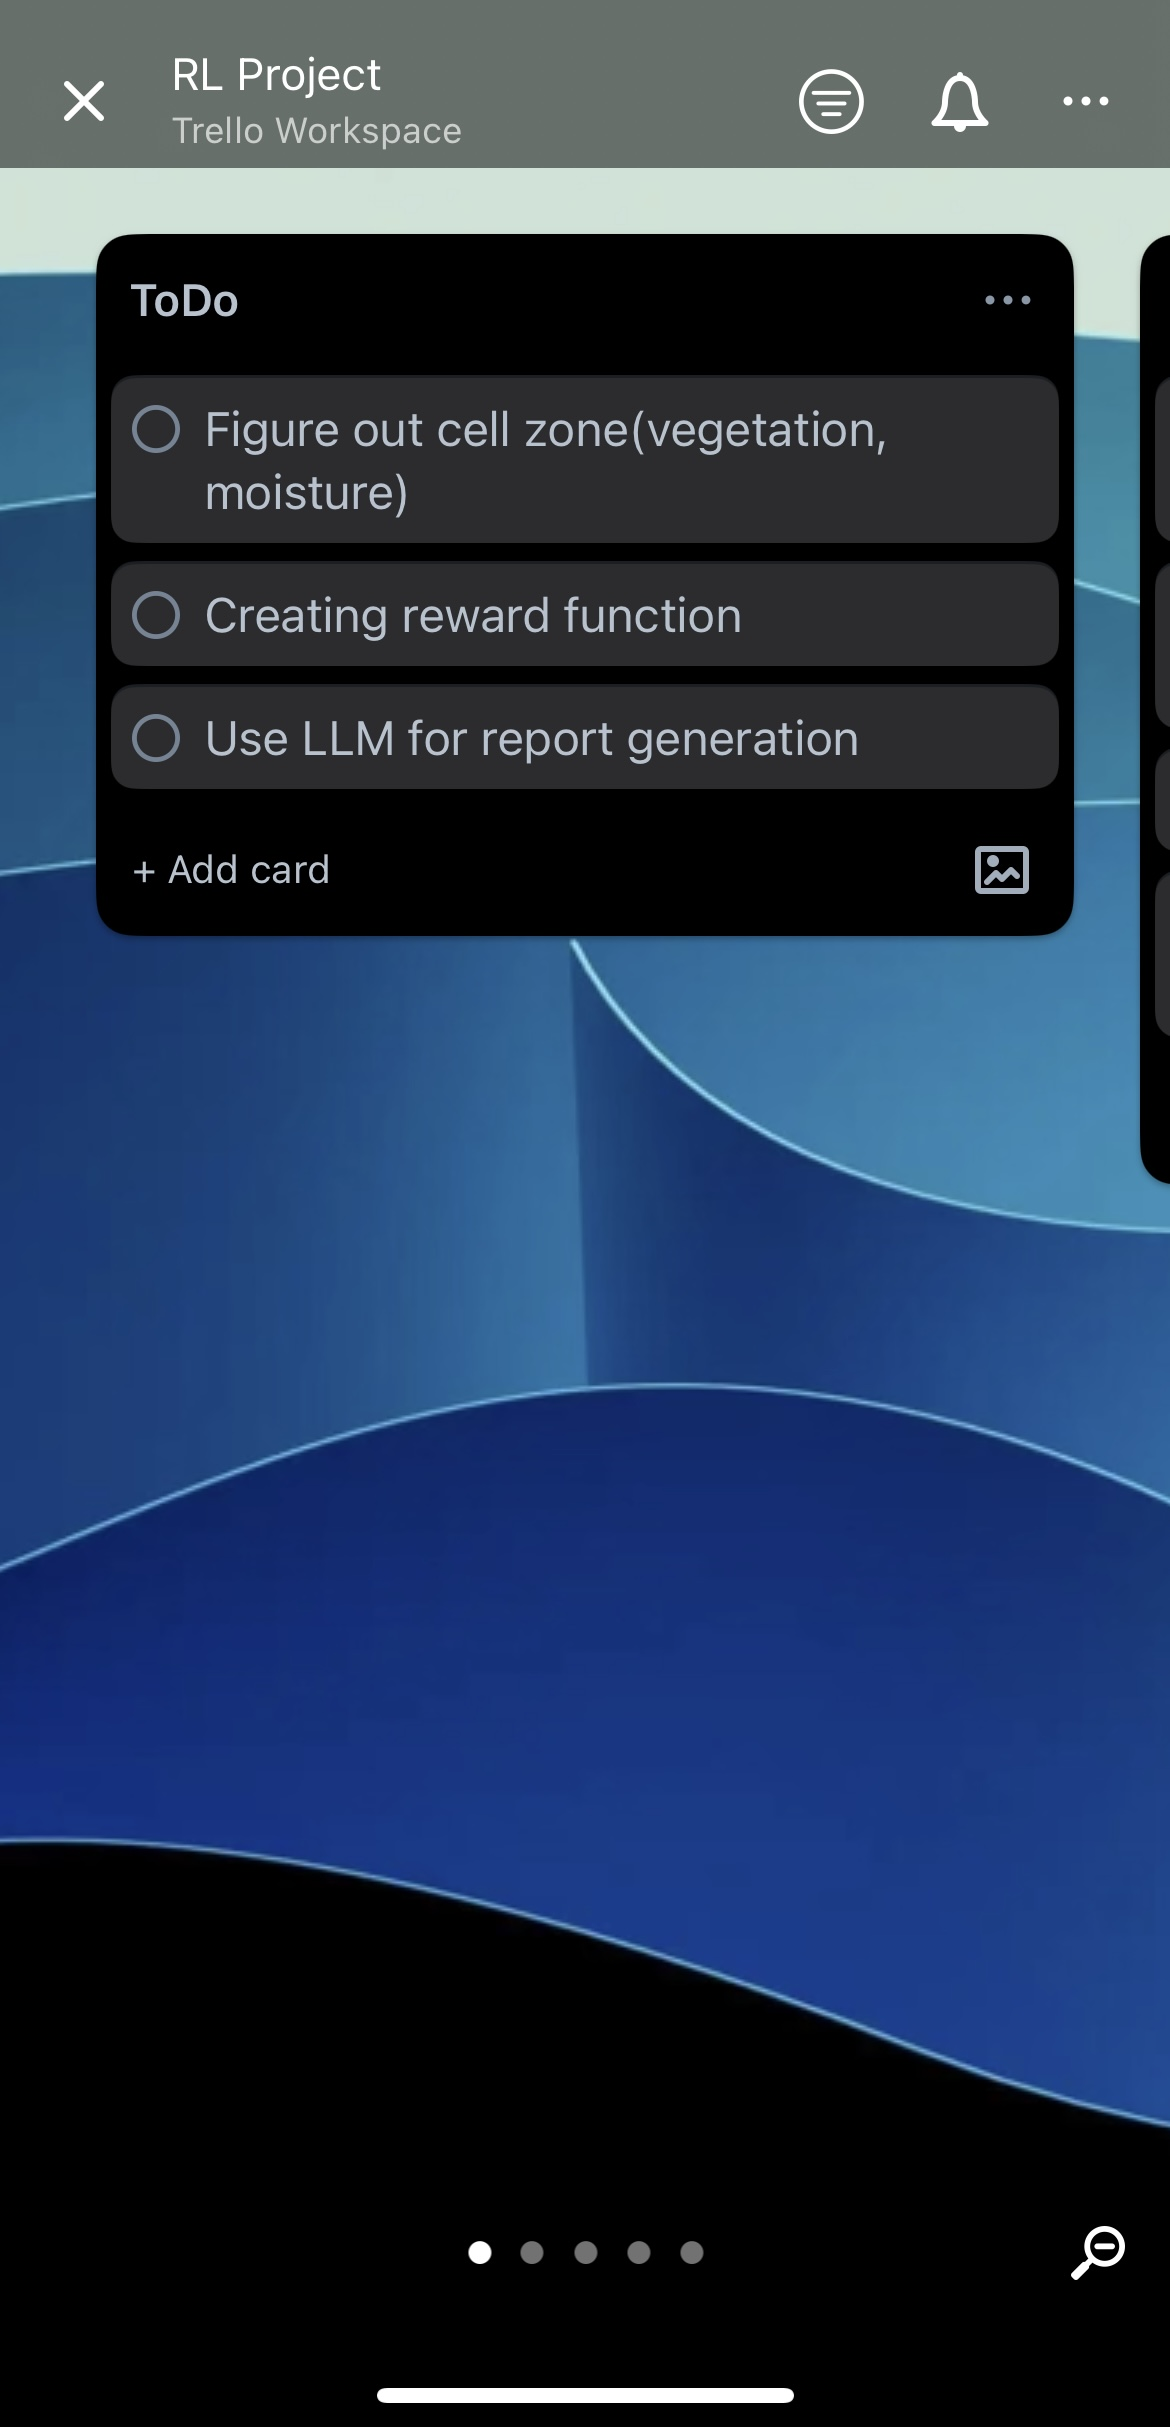
\includegraphics[width=0.22\textwidth]{5.jpg}
\end{figure}

\vspace{-0.3cm}
\noindent\textbf{Trello Board URL:} \\
\texttt{https://trello.com/b/pBNt9VwL/rl-project}

\vspace{0.3cm}
\noindent\textbf{GitHub Repository:} \\
\texttt{https://github.com/ShauryaMathur/inferno-tactix/tree/wildfire-env}

\subsection{GitHub Commit History}
\hspace{-0.4cm}Below is a snapshot of our git commit history demonstrating ongoing collaboration and iterative development:

\begin{figure}[H]
\centering
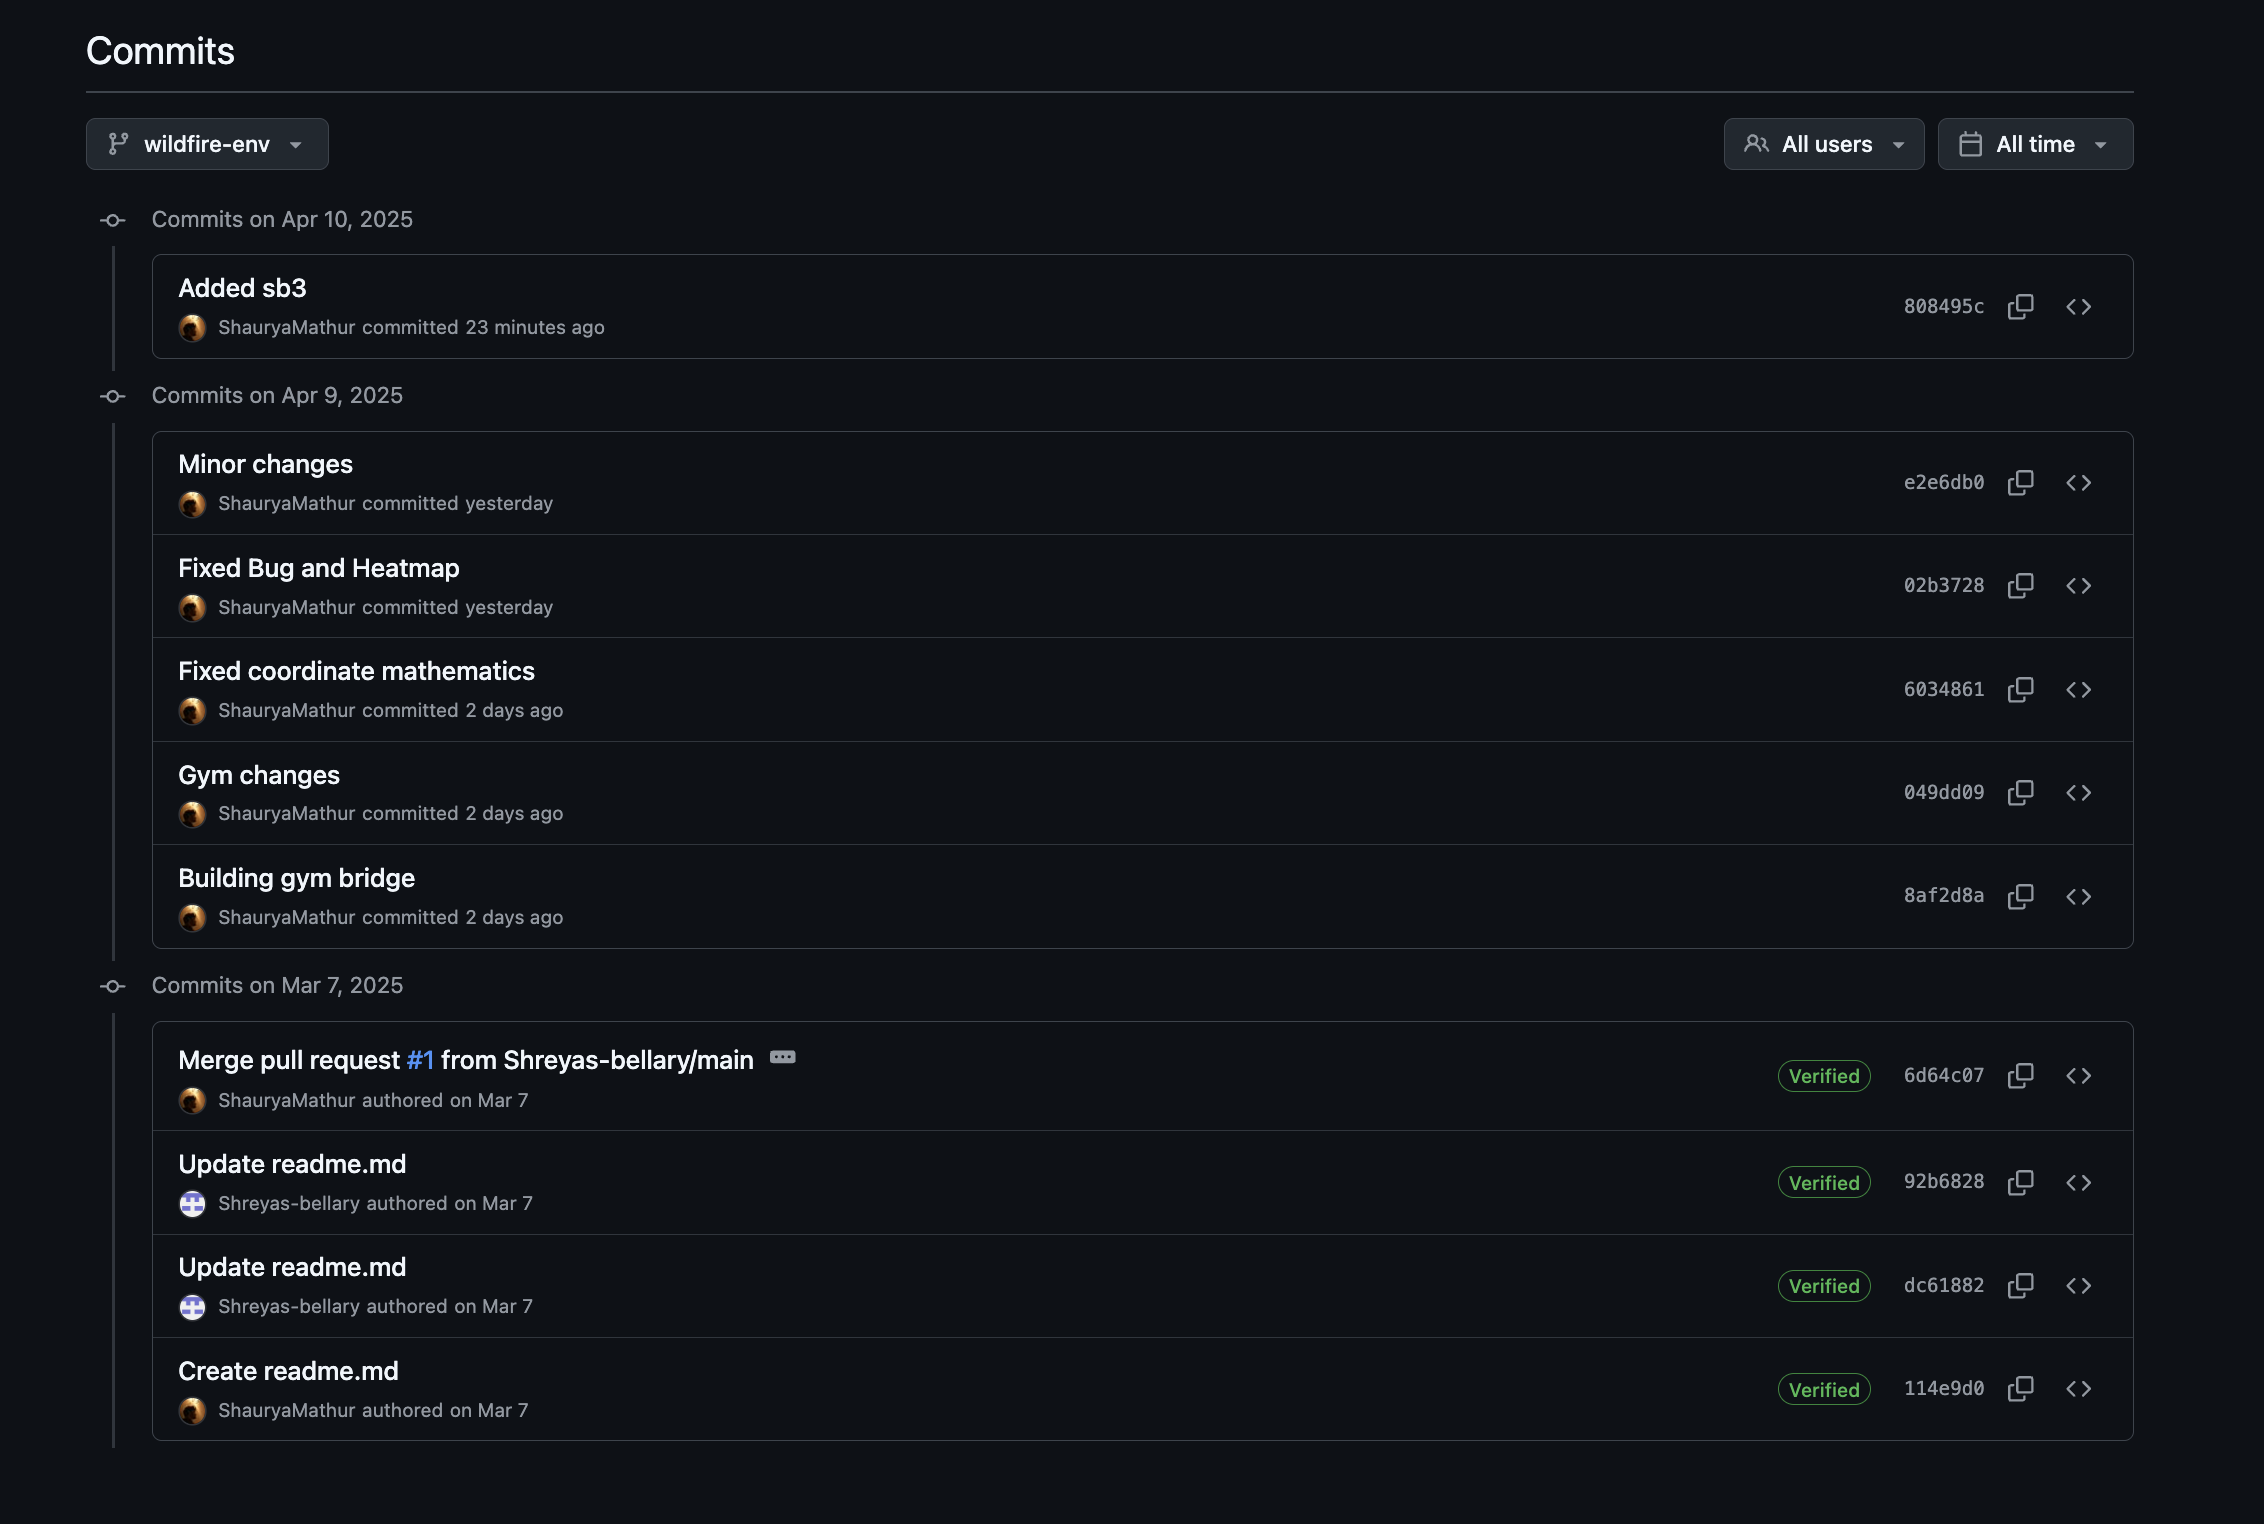
\includegraphics[width=0.75\textwidth]{6.png} 
\caption{git commit history}
\end{figure}


\vspace{0.4cm}
\begin{thebibliography}{00}
\bibitem{b1} https://github.com/amanbasu/wildfire-detection.
\bibitem{b2} https://code.earthengine.google.com/
\bibitem{b3} https://wildfire.concord.org/
\bibitem{b4} https://github.com/concord-consortium/wildfire-model/tree/master
\bibitem{b5} U.S. Geological Survey, \emph{Landsat 8 (L8) Data Users Handbook}, U.S. Geological Survey, 2019. [Online]. Available: \url{https://landsat.usgs.gov/landsat-8}
\bibitem{b6} Y. Zhao, M. Chen, and S. Kumar, ``A Comprehensive Review of Deep Learning Techniques for Wildfire Detection in Satellite Images,'' \emph{IEEE Access}, vol. 9, pp. 10523--10539, 2021.
\bibitem{b7} M. Pereira and G. H. A., ``Active Fire Detection in Landsat-8 Imagery: A Large-Scale Dataset,'' GitHub, 2023. [Online]. Available: \url{https://github.com/pereira-gha/activefire}
\end{thebibliography}

\end{document}
